\section{Результаты}
\begin{enumerate}[noitemsep, topsep=0pt]
	\item Отразить в виде таблички или графиков замеры времени работы ядер с различными конфигурациями (начиная с <{}<{}< 1, 32 >{}>{}> и как минимум до <{}<{}< 1024, 1024 >{}>{}>) и различными входными данными (небольшие тесты, средние и предельные). \\
	\item Произвести сравнение с CPU (для этого нужно реализовать свой вариант ЛР без использования технологии CUDA). Время на копирование входных-выходных данных не учитывать, замерять только время работы самого алгоритма. \\
	\item Если программа подразумевает работу с изображениями, то необходимо наличие скриншотов.
\end{enumerate}

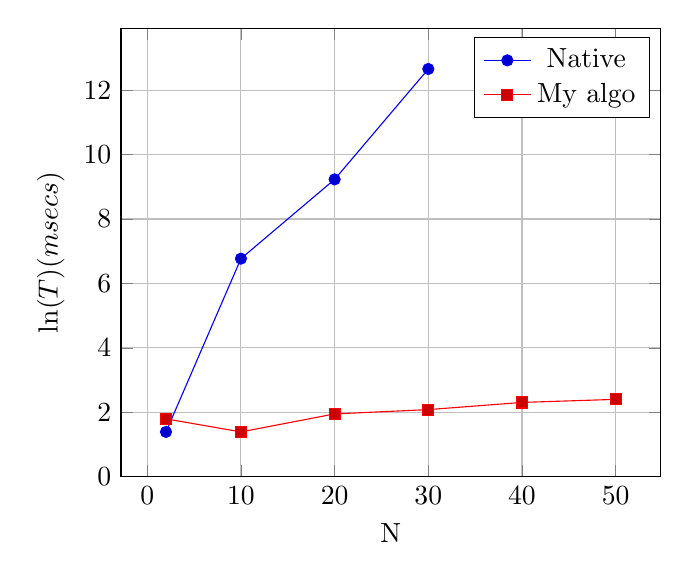
\begin{tikzpicture}% coordinates
	\begin{axis}[
		xlabel=N,
		ylabel= $\ln(T) (msecs)$,
		ymin = 0,
		grid=major
		]
		\legend{Native, My algo}
		\addplot coordinates {(2, 1.3862943611199) (10, 6.7696419768525) (20, 9.2319061498907) (30, 12.661704747321)};
		\addplot coordinates {(2, 1.7917594692281) (10, 1.3862943611199) (20, 1.9459101490553) (30, 2.0794415416798) (40, 2.302585092994) (50, 2.3978952727984)};
	\end{axis}
\end{tikzpicture}